\documentclass{report}
\usepackage[utf8]{inputenc}
\usepackage{tabularx}
\usepackage{graphicx}
\usepackage{verbatim}
\usepackage{xcolor}
\usepackage{tikz,pgfplots}
\usepackage{circuitikz}
\usepackage{fixlatvian}
\title{1.laboratorijas darbs."Vienkāršu elektrisku shēmu modelēšana"}
\author{Ruslans Babajans}
\date{Marts 2018}
\begin{document}

\maketitle
\chapter{Teorētiskā daļa}
\section{Ķēdes aprēķins}
Darba uzdevums bija apreķināt spriegumus uz rezistoriem. Sprieguma avota V1 sprieguma vērtība U (Voltos) $V1 = 15.2 V$ ,$R1={6} \Omega$,$R2={3} \Omega$.
Tā kā shēmā bija virknes slēgums, tika izmantota sprieguma dalītāja formula\newline $U1=(R1/(R1+R2))*V1$
Līdzīgi $U2=(R2/(R1+R2))*V1$
\begin{figure}[!h]
\centering
\begin{tabular}{|c|c|}
\hline
R1 & $6 \Omega$ \\
\hline
R2 & $3 \Omega$ \\
\hline
V1 & 15.2 V \\
\hline
U1 & 10.2 V\\
\hline
U2 &  5 V\\
\hline
\end{tabular}
\end{figure}

\begin{figure}[b]
\centering
\begin{circuitikz}[american voltages]
\draw (8,2)
      to[V=$U_s$] (8,6)
      to[R=$R_1$] (12,6)
      to[R=$R_2$] (12,2)
      to[short] (8,2);
\end{circuitikz}
\caption{Sprieguma dalītāja shēma}
\end{figure}

\begin{figure}[t!]
\centering
\begin{tikzpicture}
\begin{axis}[
        axis lines= middle,
        ylabel=$U2_V$,
        xlabel=$R2_\Omega$,
        ymin=0,
        minor y tick num=1,
        minor x tick num=1,]

\addplot[
    thick,
    blue,
    domain=0:15,
    samples=100,]
{(x*15.2)/(6+x)};
\end{axis}
\end{tikzpicture}
\caption{shēmas UR2=f(R2) grafiks}
\end{figure}

\chapter{Praktiskā daļa}
\section{Darbs ar GEDA programmām}
\subsection{Darbs ar gschem}

\begin{figure}[!b]
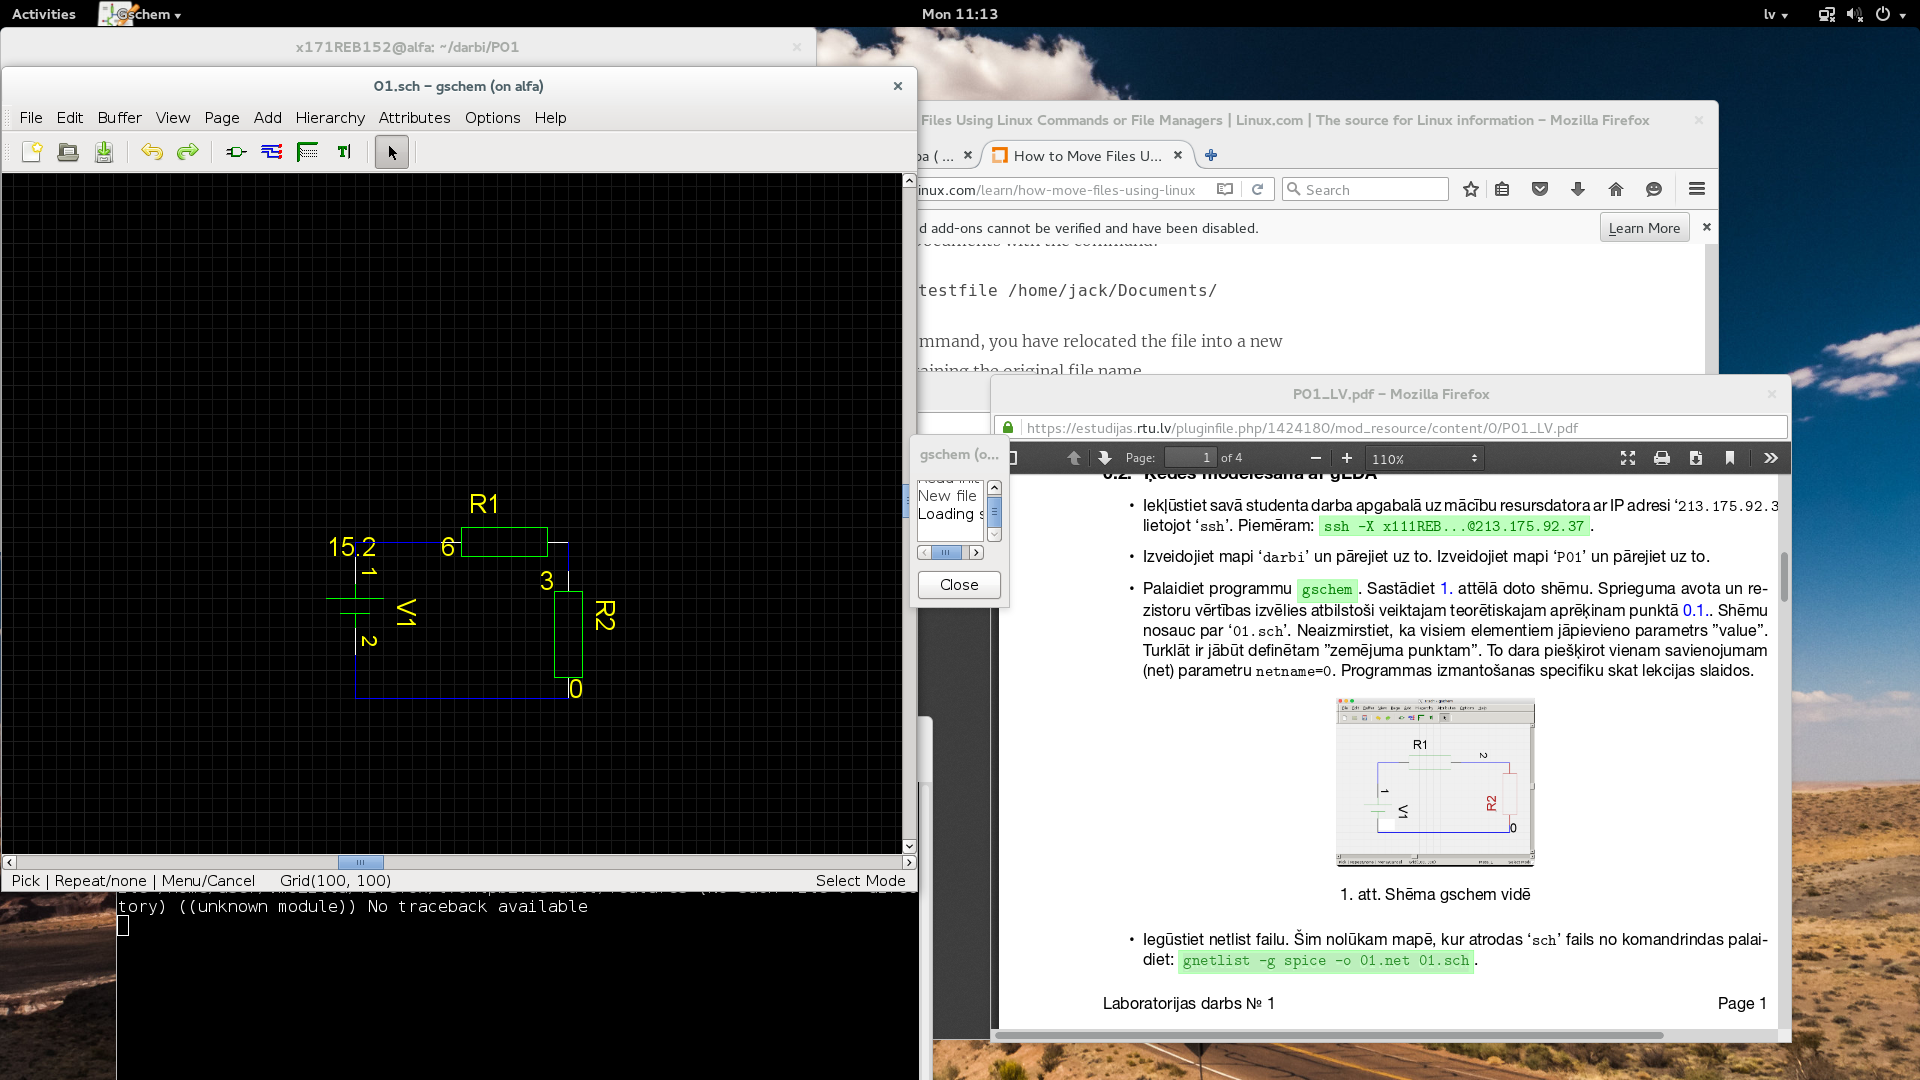
\includegraphics[width=14cm]{bildes/01.png}
\caption{Ar Gschem izveidotā shēma}
\label{1}
\end{figure}
\newpage
\subsection{Dards ar gnetlist}
\begin{verbatim}
* Spice netlister for gnetlist
R2 2 0 3
R1 1 2 6
V1 1 0 15.2
.END
\end{verbatim}

\subsection{Darbs ar ngspice}

\begin{figure}[!b]
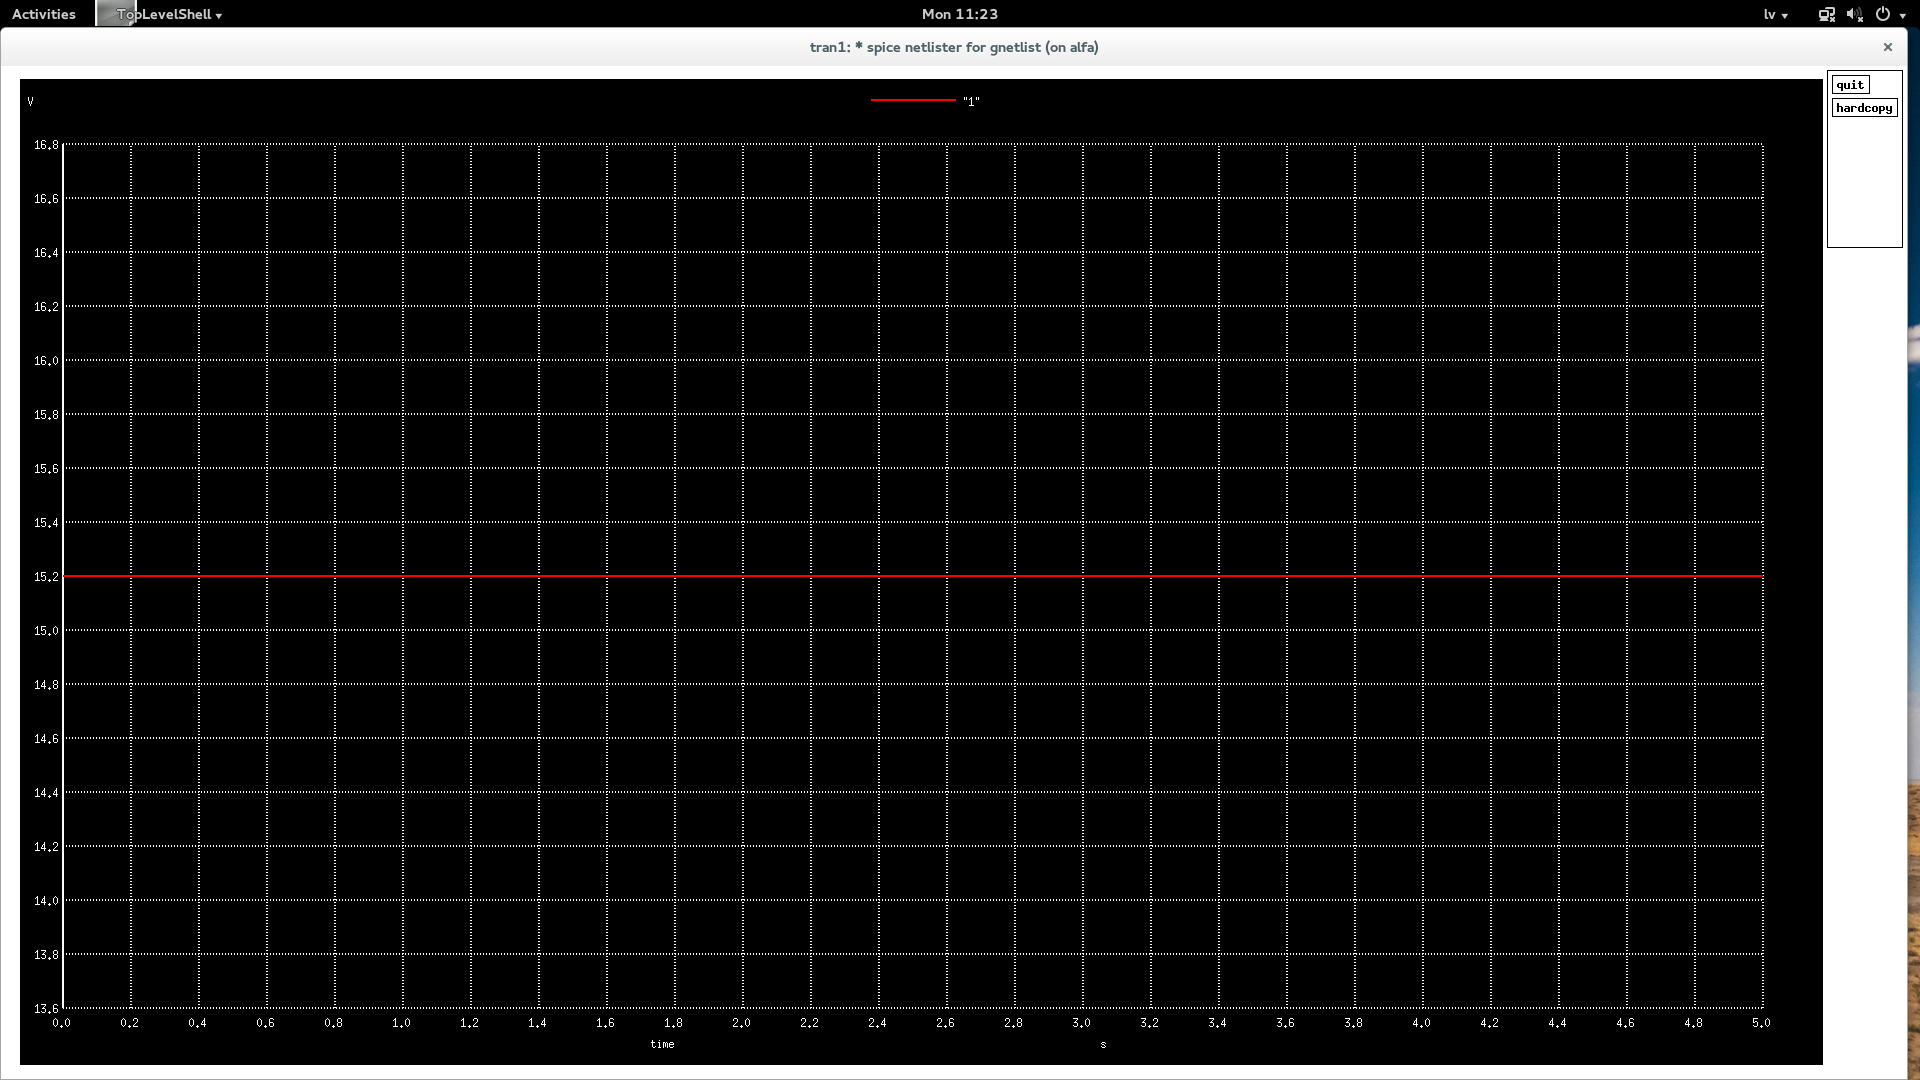
\includegraphics[width=11cm]{bildes/011.png}
\caption{UR1}
\label{2}
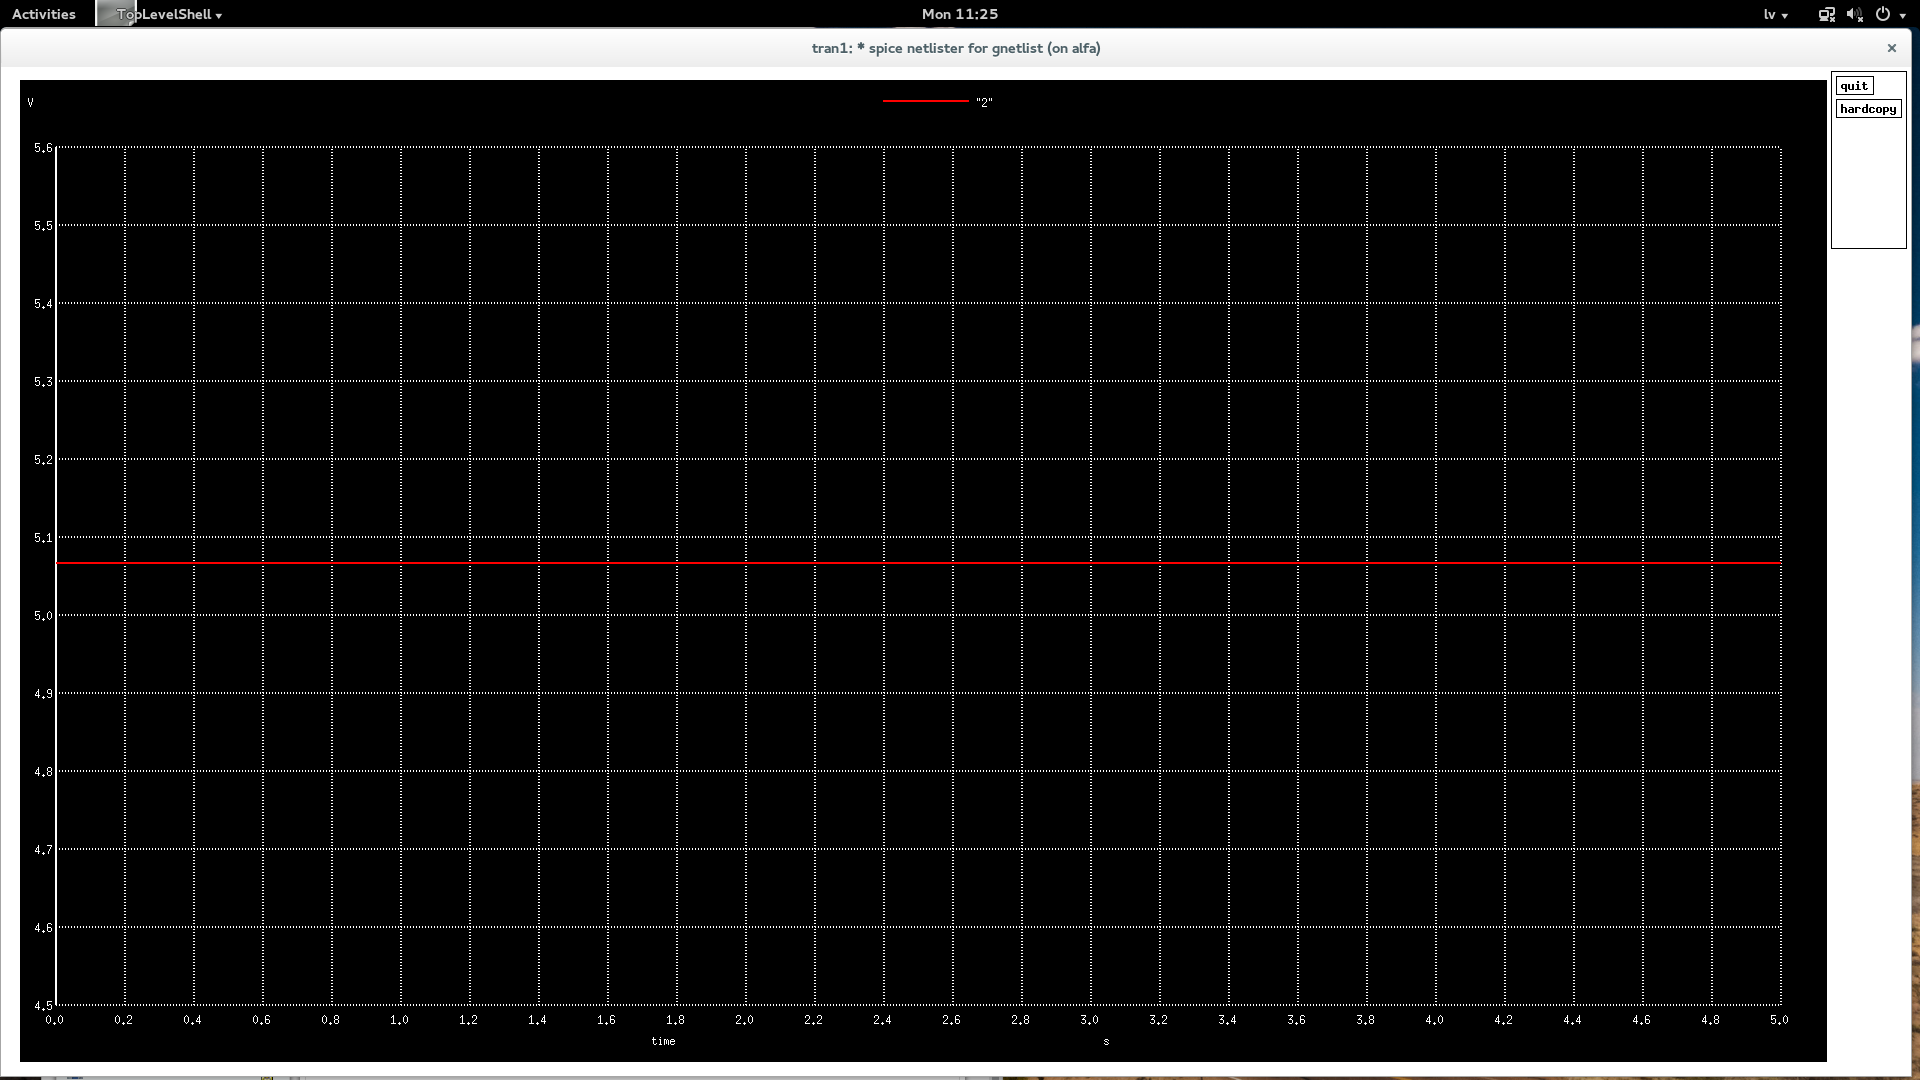
\includegraphics[width=11cm]{bildes/012.png}
\caption{UR2}
\label{3}
\end{figure}
\newpage
\section{Darbs ar QUCS programmām}

\begin{figure}[!b]
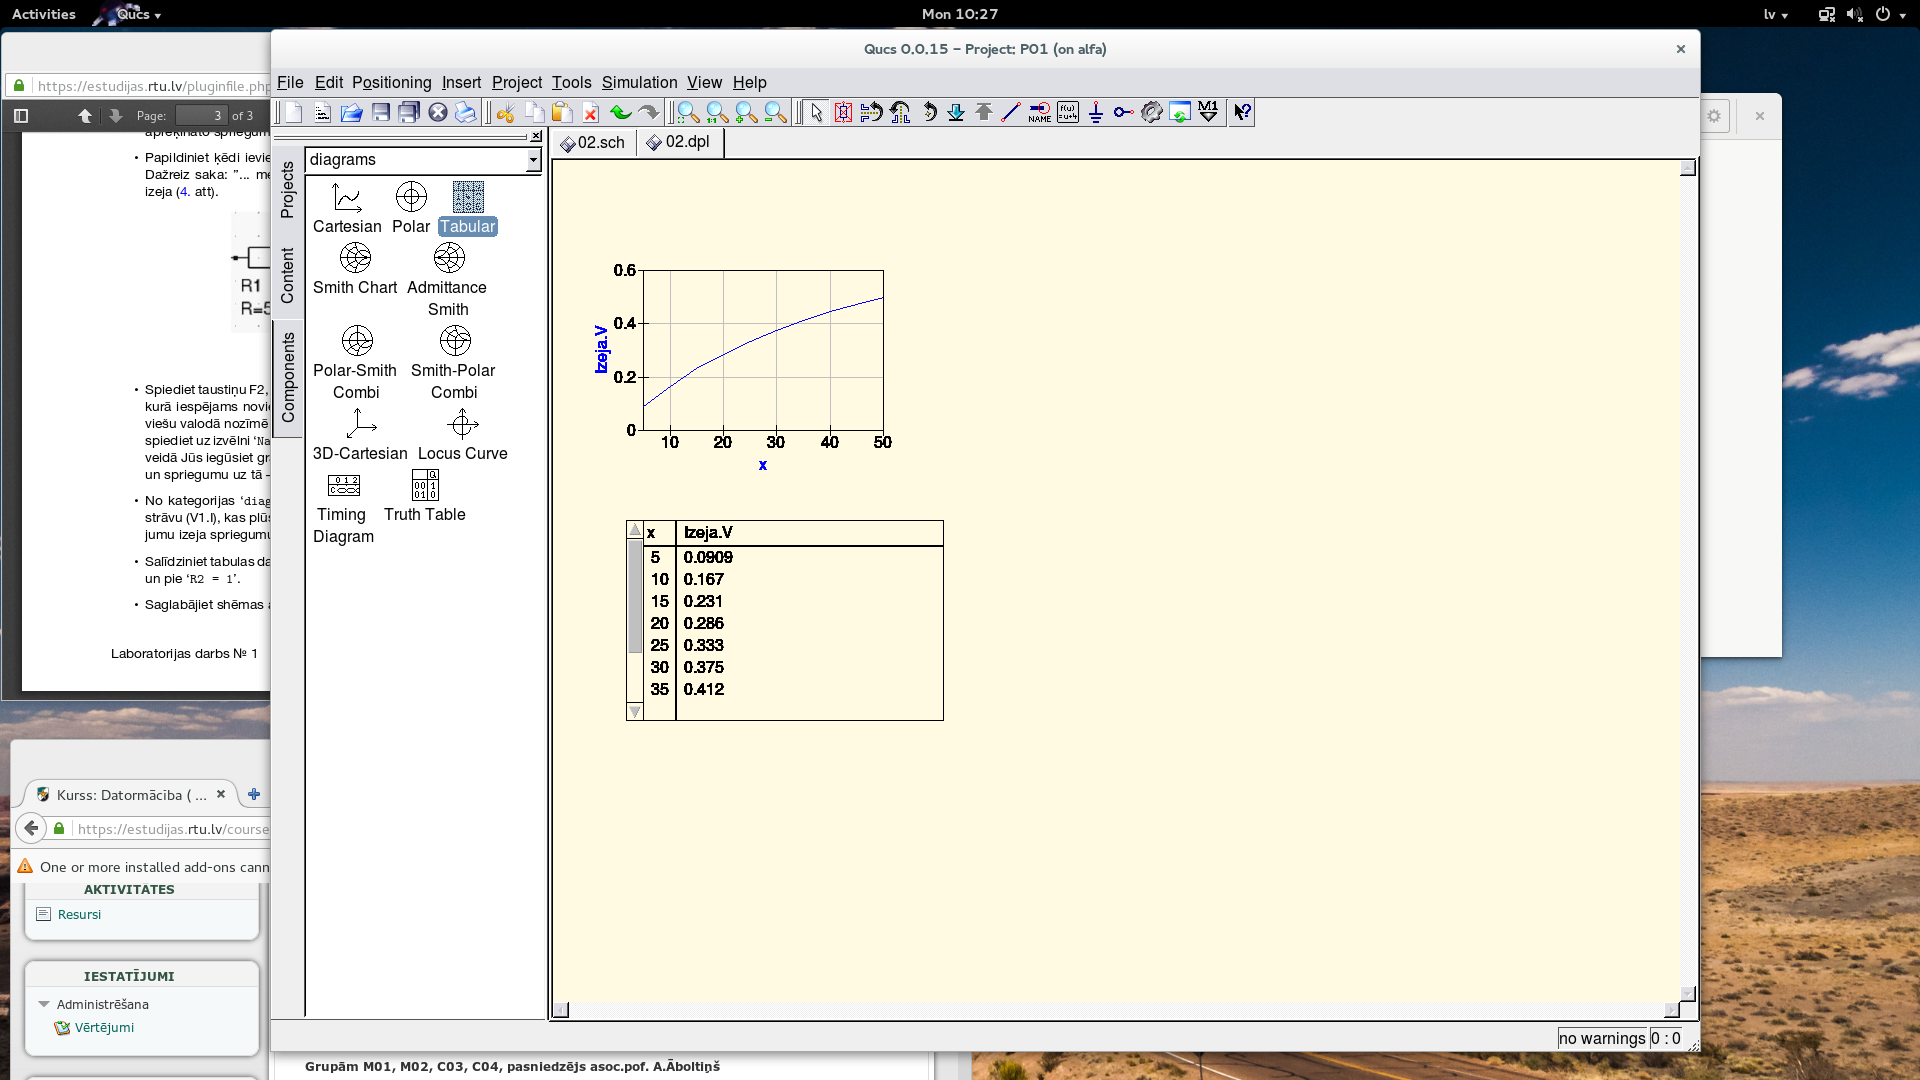
\includegraphics[width=13cm]{bildes/qucs1.png}
\caption{Sweep simulācijas grafiks un tābula}
\label{4}
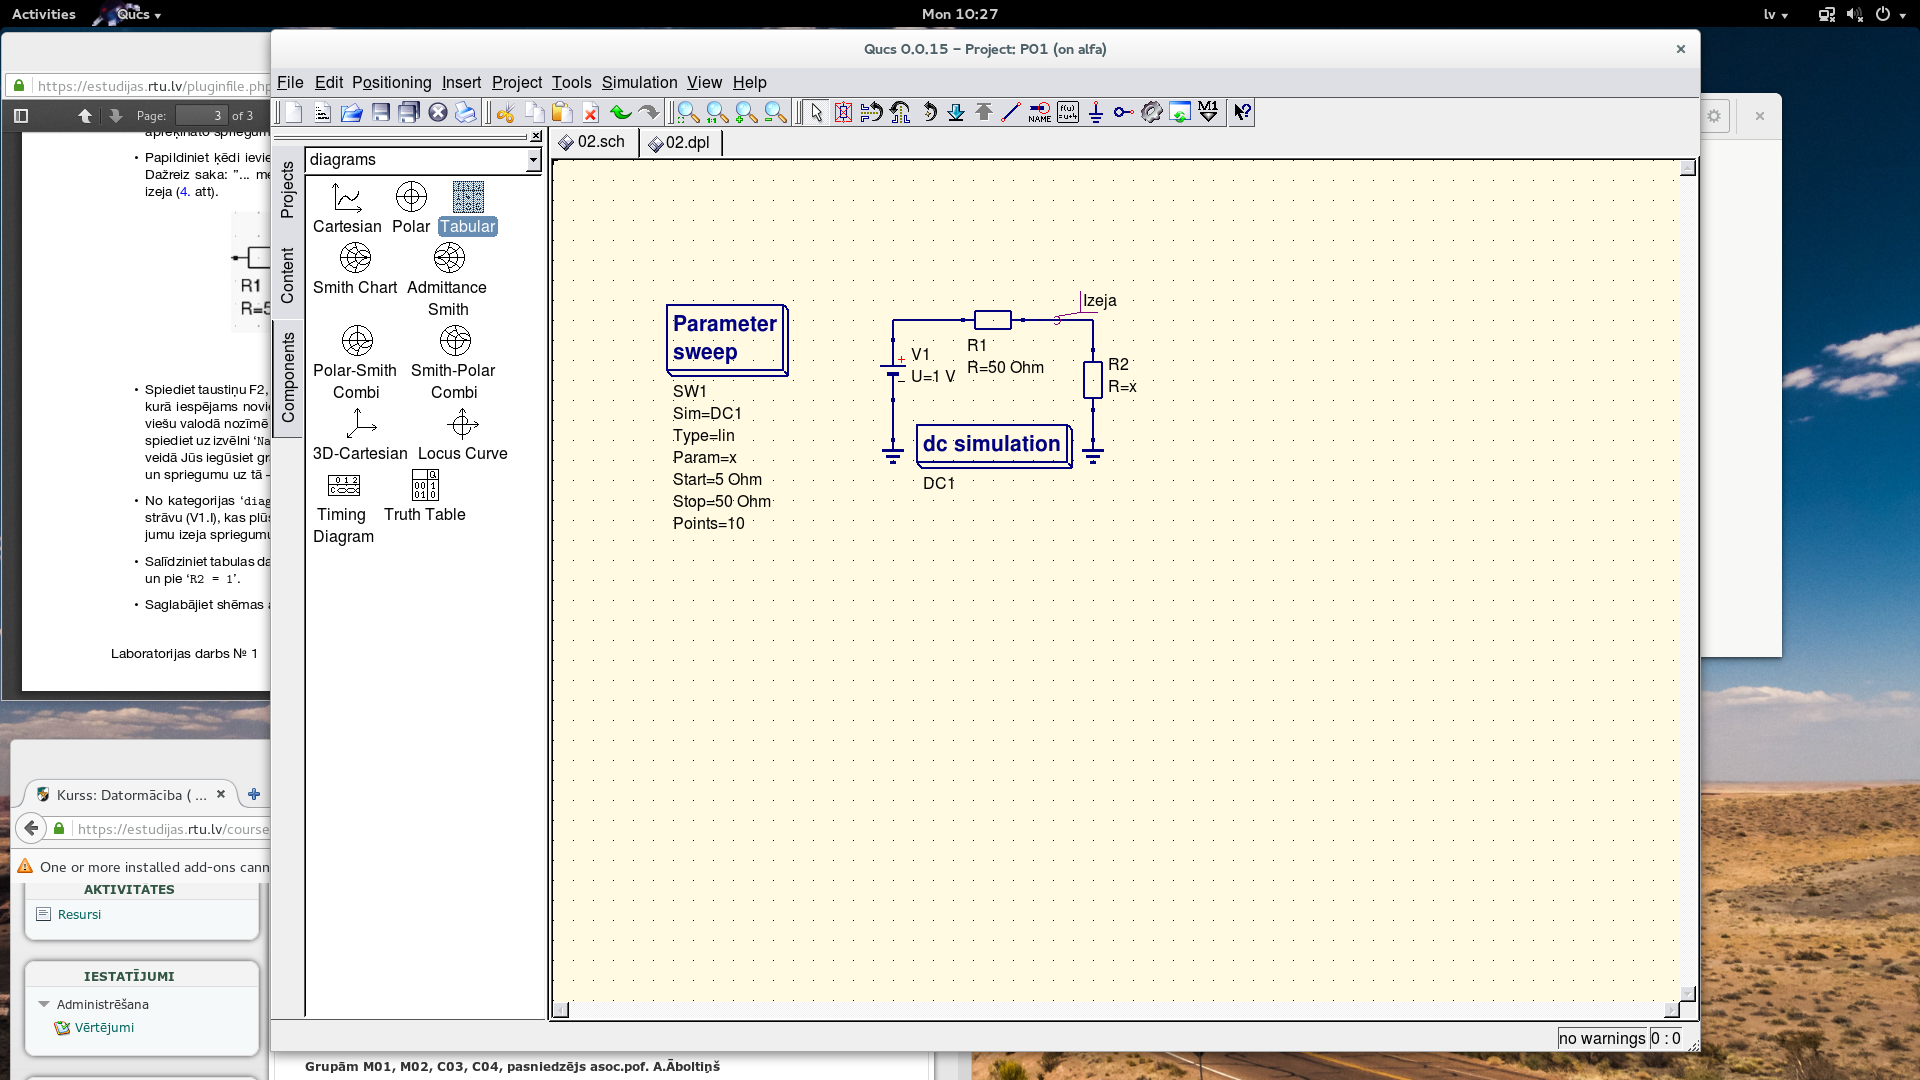
\includegraphics[width=13cm]{bildes/qucs2.png}
\caption{Principiālā shēma}
\label{5}
\end{figure}

\chapter{Atsauksmes}
Veicot šo darbu tika izmantota informācija no \cite{1} shēmas zimēšanai un \cite{2} figūras floata pareizai pielietošanai.

\begin{thebibliography}{2}
\bibitem{1}\texttt{$https://www.sharelatex.com/learn/CircuiTikz_package$}
\bibitem{2}\texttt{$https://www.sharelatex.com/learn/Positioning_of_Figures$}

\end{thebibliography}
\end{document}
